\chapter{Introduction}
\label{ch:introduction}

Type~1 diabetes mellitus is an autoimmune condition in which the immune system destroys the insulin-producing beta cells of the pancreas, eliminating endogenous insulin secretion and necessitating lifelong external insulin administration~\citep{dimeglio2018t1d}. The global scale of the condition is substantial: the IDF Diabetes Atlas reports that approximately 537 million adults were living with diabetes in 2021~\citep{idf2021atlas}, with Type~1 accounting for a considerable proportion of paediatric and young-adult cases. Managing blood glucose within safe limits is a continuous and technically demanding task for patients and clinicians alike.

Continuous glucose monitoring (CGM) devices address this challenge by measuring interstitial glucose every five minutes, providing a dense real-time signal that serves as the foundational input for modern automated insulin delivery systems~\citep{bekiari2018aid}. A critical clinical target is the hypoglycaemia threshold of 70~mg/dL: glucose values below this level can rapidly progress to seizures, loss of consciousness, and, in severe cases, death~\citep{battelino2019}. Pharmacodynamic delays of 15 to 45 minutes between an insulin dose and its glycaemic effect~\citep{hovorka2011closedloop} mean that a hypoglycaemia event must be anticipated in advance to allow timely intervention. A missed event carries far greater clinical risk than a false alarm~\citep{battelino2019}, which motivates the use of recall-weighted evaluation metrics; the F2 score used throughout this thesis is formally introduced in Section~\ref{sec:bg:metrics}.

Deep learning models trained with mean squared error on the glucose signal systematically produce predictions that are structurally correct but displaced forward in time by approximately 50 to 55~minutes, an effect first observed in preliminary PRG experiments~\citep{prg_glucose_proposal}. The root cause is mathematical: the CGM signal exhibits strong lag-1 autocorrelation (Section~\ref{sec:method:setup:cgm}), meaning the glucose value one step ahead is nearly identical to the current value. MSE training therefore rewards a model that reproduces recent glucose history rather than learning to anticipate future changes, because copying the past incurs almost no penalty under a pointwise loss~\citep{wolff2025cgpm}. The result is a prediction curve that mirrors the true trajectory at a temporal offset, as illustrated in Fig.~\ref{fig:intro:timeshift_demo}.

The clinical consequence is direct: if the predicted threshold crossing occurs 50~minutes after the true one, the derived alarm fires after the patient has already become hypoglycaemic. Forecast-derived event detection therefore fails not because the model is structurally unable to represent future glucose behaviour, but because its output is displaced in time. Separating this timing component from genuine shape inaccuracy requires a lag-adjusted evaluation metric that measures the prediction error remaining after the systematic shift has been removed; it is defined formally in Section~\ref{sec:bg:metrics}.

\begin{figure}[tbp]
    \centering
    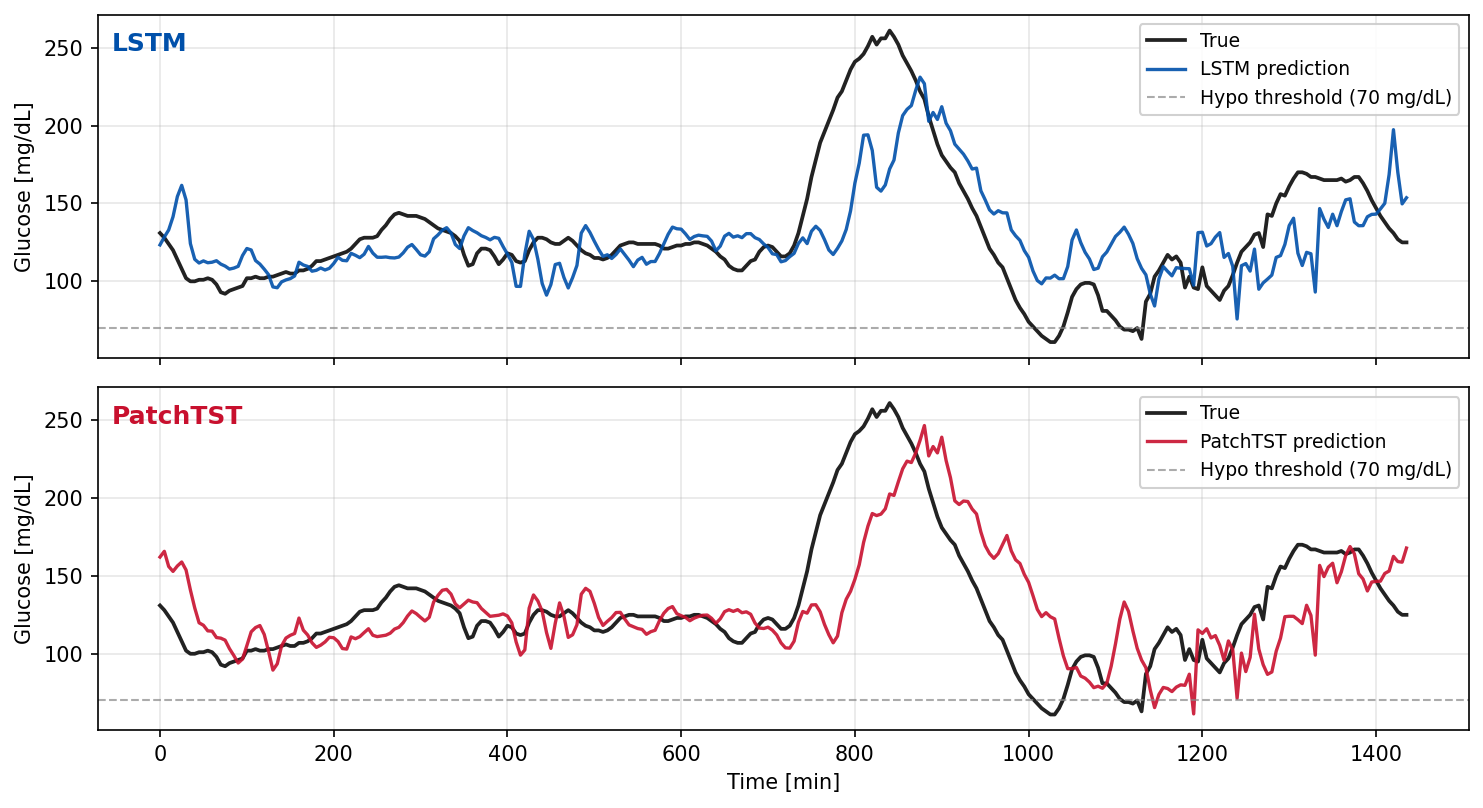
\includegraphics[width=0.9\textwidth]{timeshift_demo.png}
    \caption[Illustration of the time-shift artefact in glucose forecasting]{%
    Illustration of the time-shift artefact in MSE-trained univariate
    glucose forecasting models. Both the LSTM (top) and PatchTST (bottom)
    predictions are plotted against the true glucose trajectory over the
    same time window. The dashed line marks the 70~mg/dL hypoglycaemia
    threshold; the region below indicates the hypoglycaemic zone.}
    \label{fig:intro:timeshift_demo}
\end{figure}

Closely related work at the University of Bern is the bachelor thesis of \citet{huni2023glucose}, which evaluated LSTM and Graph Attention Networks for hypoglycaemia prediction on CGM data. That study did not isolate or quantify the time-shift artefact as a distinct phenomenon, which is the primary focus of the present work. At the architecture level, \citet{lim2021tsforecast} survey deep learning for time-series forecasting and document the progression from recurrent models to attention-based architectures~\citep{vaswani2017attention}. PatchTST~\citep{nie2023patchtst} extends this line of work by treating fixed-length patches as attention tokens and uses Reversible Instance Normalisation~\citep{kim2022revin} to normalise each input window and counter the non-stationarity of the signal; the structural consequences of this normalisation strategy for threshold-based classification are analysed in Section~\ref{sec:exp:obj3}.

In the blood glucose domain, \citet{fox2018multioutput} demonstrate that supervising on the full future trajectory rather than a single endpoint improves forecast accuracy, forming the basis of Objective~2. For direct event detection, \citet{shao2024hypoglycemia} and \citet{cinar2025hypoclassification} show that end-to-end binary classifiers outperform threshold-based regression detection, motivating Objective~3. Regarding the time-shift specifically, \citet{wolff2025cgpm} demonstrate that accuracy-based metrics such as RMSE reward trivial models that merely reproduce the most recent observation, and argue on this basis for evaluation criteria beyond accuracy. Their contribution is diagnostic: it establishes that the delay is a real and under-recognised problem, but does not evaluate training-level strategies for reducing it. \citet{sun2026futureaware} address the prediction delay through future-aware training that injects privileged future-disturbance information during training, a different intervention from the offset-aware and event-centric strategies examined here. The present thesis takes the problem identified by these works as its starting point and contributes what they do not: a controlled ablation of concrete mitigation strategies, evaluated with a dedicated lag-adjusted metric (RMSE$^*$) that isolates the timing component of the error from genuine shape inaccuracy.

The experiments are conducted on the T1DATA cohort~\citep{garciatirado2023t1d}, comprising CGM records from 36 anonymised adults with Type~1 diabetes recorded over approximately 30 days per patient using Dexcom G6 devices. All models are trained and evaluated independently per patient; cohort means are reported throughout. Two architectures serve as parallel baselines: a recurrent Long Short-Term Memory network and the patch-based PatchTST Transformer. A strictly univariate input is used throughout to deliberately isolate the temporal predictive capacity of the glucose signal itself. Exactly one configuration variable is modified per research objective, enabling clean attribution of any observed differences in performance.

Three research questions, identified in the PRG proposal~\citep{prg_glucose_proposal} and operationalised here as a controlled ablation study, guide the investigation:

\begin{enumerate}
    \item \textbf{Objective~1 (offset-aware loss functions):} Do the Bounded-Lag loss and Soft-DTW reduce the systematic prediction delay, and if so, does any such reduction improve hypoglycaemia event detection?
    \item \textbf{Objective~2 (multi-step supervision):} Does supervising the model on the complete future trajectory rather than a single endpoint reduce the prediction delay and improve detection performance?
    \item \textbf{Objective~3 (direct event classification):} Do task-specific binary classifiers trained end-to-end on event labels outperform threshold-based detectors derived from regression outputs?
\end{enumerate}

This thesis makes the following contributions in addressing these questions:

\begin{itemize}
    \item A controlled ablation study evaluating three strategies for mitigating the systematic prediction delay across a 36-patient cohort, with exactly one training variable changed per objective.
    \item Application of the lag-adjusted RMSE (RMSE$^*$) as a diagnostic metric that isolates the timing component of prediction error from structural shape inaccuracy.
    \item A tolerance-window sweep protocol ($\tau \in \{0, 5, \ldots, 60\}$~minutes) that characterises how much of the detection failure is attributable to timing mismatch rather than structural inability to anticipate events.
    \item Empirical evidence that glucose trajectory forecasting and hypoglycaemia event detection are best treated as separate tasks, and that the performance ranking of architectures inverts between the two tasks.
\end{itemize}

Chapter~\ref{ch:background} establishes the theoretical foundations: the LSTM and PatchTST architectures, the evaluated loss functions, and the evaluation metrics. Chapter~\ref{ch:method} defines the mathematical problem formulation, describes the T1DATA dataset, and specifies the three training objectives of the ablation study. Chapter~\ref{ch:experiments} presents the empirical results for each objective and an overall comparative summary across all ten model configurations. Chapter~\ref{ch:conclusions} summarises the findings, identifies methodological limitations, and outlines directions for future research.
